\begin{figure}[htbp]
\centering
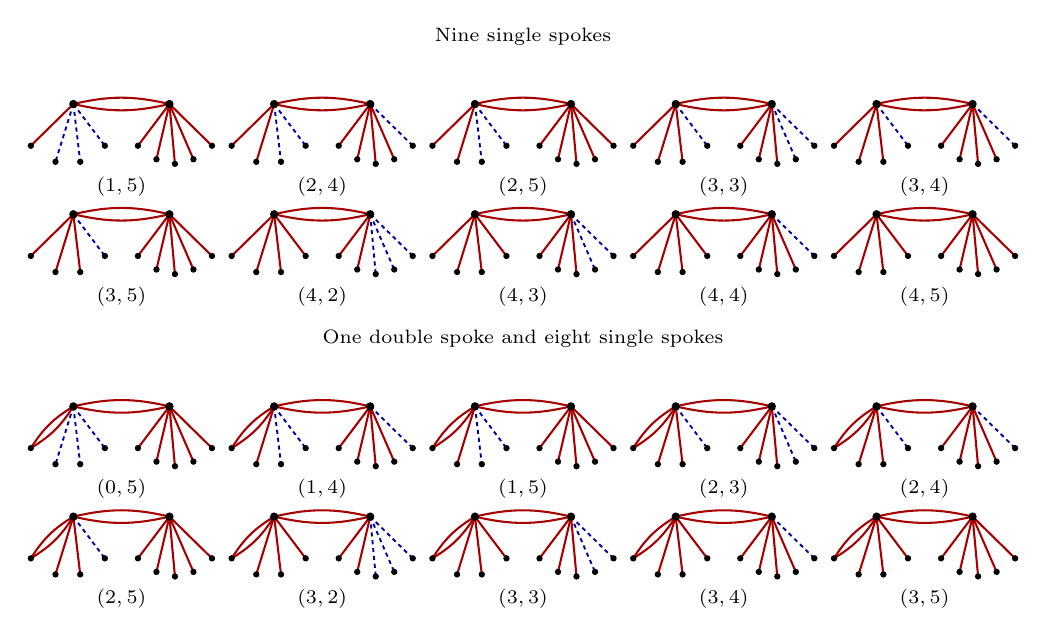
\begin{tikzpicture}[font=\scriptsize,
sc marked/.style={draw=red!65!black,line width=.75pt},
sc unmarked/.style={draw=blue!65!black,line width=.68pt,dash pattern=on 1.5pt off 1.35pt}]
\node[inner sep=0pt] at (0,0) {Nine single spokes};
\begin{scope}[shift={(-5.1,-0.89)}]
\coordinate (u) at (-0.61,0.03);
\coordinate (v) at (0.61,0.03);
\coordinate (u0) at (-1.15,-0.5);
\coordinate (u1) at (-0.837,-0.704);
\coordinate (u2) at (-0.523,-0.704);
\coordinate (u3) at (-0.21,-0.5);
\coordinate (v0) at (0.21,-0.5);
\coordinate (v1) at (0.445,-0.672);
\coordinate (v2) at (0.68,-0.73);
\coordinate (v3) at (0.915,-0.672);
\coordinate (v4) at (1.15,-0.5);
\draw[sc marked] (u) to[bend left=13] (v);
\draw[sc marked] (u) to[bend right=13] (v);
\draw[sc marked] (u) -- (u0);
\draw[sc unmarked] (u) -- (u1);
\draw[sc unmarked] (u) -- (u2);
\draw[sc unmarked] (u) -- (u3);
\draw[sc marked] (v) -- (v0);
\draw[sc marked] (v) -- (v1);
\draw[sc marked] (v) -- (v2);
\draw[sc marked] (v) -- (v3);
\draw[sc marked] (v) -- (v4);
\fill (u) circle[radius=1.5pt];
\fill (v) circle[radius=1.5pt];
\fill (u0) circle[radius=1.15pt];
\fill (u1) circle[radius=1.15pt];
\fill (u2) circle[radius=1.15pt];
\fill (u3) circle[radius=1.15pt];
\fill (v0) circle[radius=1.15pt];
\fill (v1) circle[radius=1.15pt];
\fill (v2) circle[radius=1.15pt];
\fill (v3) circle[radius=1.15pt];
\fill (v4) circle[radius=1.15pt];
\node[anchor=north,inner sep=1pt] at (0,-.85) {\((1,5)\)};
\end{scope}
\begin{scope}[shift={(-2.55,-0.89)}]
\coordinate (u) at (-0.61,0.03);
\coordinate (v) at (0.61,0.03);
\coordinate (u0) at (-1.15,-0.5);
\coordinate (u1) at (-0.837,-0.704);
\coordinate (u2) at (-0.523,-0.704);
\coordinate (u3) at (-0.21,-0.5);
\coordinate (v0) at (0.21,-0.5);
\coordinate (v1) at (0.445,-0.672);
\coordinate (v2) at (0.68,-0.73);
\coordinate (v3) at (0.915,-0.672);
\coordinate (v4) at (1.15,-0.5);
\draw[sc marked] (u) to[bend left=13] (v);
\draw[sc marked] (u) to[bend right=13] (v);
\draw[sc marked] (u) -- (u0);
\draw[sc marked] (u) -- (u1);
\draw[sc unmarked] (u) -- (u2);
\draw[sc unmarked] (u) -- (u3);
\draw[sc marked] (v) -- (v0);
\draw[sc marked] (v) -- (v1);
\draw[sc marked] (v) -- (v2);
\draw[sc marked] (v) -- (v3);
\draw[sc unmarked] (v) -- (v4);
\fill (u) circle[radius=1.5pt];
\fill (v) circle[radius=1.5pt];
\fill (u0) circle[radius=1.15pt];
\fill (u1) circle[radius=1.15pt];
\fill (u2) circle[radius=1.15pt];
\fill (u3) circle[radius=1.15pt];
\fill (v0) circle[radius=1.15pt];
\fill (v1) circle[radius=1.15pt];
\fill (v2) circle[radius=1.15pt];
\fill (v3) circle[radius=1.15pt];
\fill (v4) circle[radius=1.15pt];
\node[anchor=north,inner sep=1pt] at (0,-.85) {\((2,4)\)};
\end{scope}
\begin{scope}[shift={(0,-0.89)}]
\coordinate (u) at (-0.61,0.03);
\coordinate (v) at (0.61,0.03);
\coordinate (u0) at (-1.15,-0.5);
\coordinate (u1) at (-0.837,-0.704);
\coordinate (u2) at (-0.523,-0.704);
\coordinate (u3) at (-0.21,-0.5);
\coordinate (v0) at (0.21,-0.5);
\coordinate (v1) at (0.445,-0.672);
\coordinate (v2) at (0.68,-0.73);
\coordinate (v3) at (0.915,-0.672);
\coordinate (v4) at (1.15,-0.5);
\draw[sc marked] (u) to[bend left=13] (v);
\draw[sc marked] (u) to[bend right=13] (v);
\draw[sc marked] (u) -- (u0);
\draw[sc marked] (u) -- (u1);
\draw[sc unmarked] (u) -- (u2);
\draw[sc unmarked] (u) -- (u3);
\draw[sc marked] (v) -- (v0);
\draw[sc marked] (v) -- (v1);
\draw[sc marked] (v) -- (v2);
\draw[sc marked] (v) -- (v3);
\draw[sc marked] (v) -- (v4);
\fill (u) circle[radius=1.5pt];
\fill (v) circle[radius=1.5pt];
\fill (u0) circle[radius=1.15pt];
\fill (u1) circle[radius=1.15pt];
\fill (u2) circle[radius=1.15pt];
\fill (u3) circle[radius=1.15pt];
\fill (v0) circle[radius=1.15pt];
\fill (v1) circle[radius=1.15pt];
\fill (v2) circle[radius=1.15pt];
\fill (v3) circle[radius=1.15pt];
\fill (v4) circle[radius=1.15pt];
\node[anchor=north,inner sep=1pt] at (0,-.85) {\((2,5)\)};
\end{scope}
\begin{scope}[shift={(2.55,-0.89)}]
\coordinate (u) at (-0.61,0.03);
\coordinate (v) at (0.61,0.03);
\coordinate (u0) at (-1.15,-0.5);
\coordinate (u1) at (-0.837,-0.704);
\coordinate (u2) at (-0.523,-0.704);
\coordinate (u3) at (-0.21,-0.5);
\coordinate (v0) at (0.21,-0.5);
\coordinate (v1) at (0.445,-0.672);
\coordinate (v2) at (0.68,-0.73);
\coordinate (v3) at (0.915,-0.672);
\coordinate (v4) at (1.15,-0.5);
\draw[sc marked] (u) to[bend left=13] (v);
\draw[sc marked] (u) to[bend right=13] (v);
\draw[sc marked] (u) -- (u0);
\draw[sc marked] (u) -- (u1);
\draw[sc marked] (u) -- (u2);
\draw[sc unmarked] (u) -- (u3);
\draw[sc marked] (v) -- (v0);
\draw[sc marked] (v) -- (v1);
\draw[sc marked] (v) -- (v2);
\draw[sc unmarked] (v) -- (v3);
\draw[sc unmarked] (v) -- (v4);
\fill (u) circle[radius=1.5pt];
\fill (v) circle[radius=1.5pt];
\fill (u0) circle[radius=1.15pt];
\fill (u1) circle[radius=1.15pt];
\fill (u2) circle[radius=1.15pt];
\fill (u3) circle[radius=1.15pt];
\fill (v0) circle[radius=1.15pt];
\fill (v1) circle[radius=1.15pt];
\fill (v2) circle[radius=1.15pt];
\fill (v3) circle[radius=1.15pt];
\fill (v4) circle[radius=1.15pt];
\node[anchor=north,inner sep=1pt] at (0,-.85) {\((3,3)\)};
\end{scope}
\begin{scope}[shift={(5.1,-0.89)}]
\coordinate (u) at (-0.61,0.03);
\coordinate (v) at (0.61,0.03);
\coordinate (u0) at (-1.15,-0.5);
\coordinate (u1) at (-0.837,-0.704);
\coordinate (u2) at (-0.523,-0.704);
\coordinate (u3) at (-0.21,-0.5);
\coordinate (v0) at (0.21,-0.5);
\coordinate (v1) at (0.445,-0.672);
\coordinate (v2) at (0.68,-0.73);
\coordinate (v3) at (0.915,-0.672);
\coordinate (v4) at (1.15,-0.5);
\draw[sc marked] (u) to[bend left=13] (v);
\draw[sc marked] (u) to[bend right=13] (v);
\draw[sc marked] (u) -- (u0);
\draw[sc marked] (u) -- (u1);
\draw[sc marked] (u) -- (u2);
\draw[sc unmarked] (u) -- (u3);
\draw[sc marked] (v) -- (v0);
\draw[sc marked] (v) -- (v1);
\draw[sc marked] (v) -- (v2);
\draw[sc marked] (v) -- (v3);
\draw[sc unmarked] (v) -- (v4);
\fill (u) circle[radius=1.5pt];
\fill (v) circle[radius=1.5pt];
\fill (u0) circle[radius=1.15pt];
\fill (u1) circle[radius=1.15pt];
\fill (u2) circle[radius=1.15pt];
\fill (u3) circle[radius=1.15pt];
\fill (v0) circle[radius=1.15pt];
\fill (v1) circle[radius=1.15pt];
\fill (v2) circle[radius=1.15pt];
\fill (v3) circle[radius=1.15pt];
\fill (v4) circle[radius=1.15pt];
\node[anchor=north,inner sep=1pt] at (0,-.85) {\((3,4)\)};
\end{scope}
\begin{scope}[shift={(-5.1,-2.29)}]
\coordinate (u) at (-0.61,0.03);
\coordinate (v) at (0.61,0.03);
\coordinate (u0) at (-1.15,-0.5);
\coordinate (u1) at (-0.837,-0.704);
\coordinate (u2) at (-0.523,-0.704);
\coordinate (u3) at (-0.21,-0.5);
\coordinate (v0) at (0.21,-0.5);
\coordinate (v1) at (0.445,-0.672);
\coordinate (v2) at (0.68,-0.73);
\coordinate (v3) at (0.915,-0.672);
\coordinate (v4) at (1.15,-0.5);
\draw[sc marked] (u) to[bend left=13] (v);
\draw[sc marked] (u) to[bend right=13] (v);
\draw[sc marked] (u) -- (u0);
\draw[sc marked] (u) -- (u1);
\draw[sc marked] (u) -- (u2);
\draw[sc unmarked] (u) -- (u3);
\draw[sc marked] (v) -- (v0);
\draw[sc marked] (v) -- (v1);
\draw[sc marked] (v) -- (v2);
\draw[sc marked] (v) -- (v3);
\draw[sc marked] (v) -- (v4);
\fill (u) circle[radius=1.5pt];
\fill (v) circle[radius=1.5pt];
\fill (u0) circle[radius=1.15pt];
\fill (u1) circle[radius=1.15pt];
\fill (u2) circle[radius=1.15pt];
\fill (u3) circle[radius=1.15pt];
\fill (v0) circle[radius=1.15pt];
\fill (v1) circle[radius=1.15pt];
\fill (v2) circle[radius=1.15pt];
\fill (v3) circle[radius=1.15pt];
\fill (v4) circle[radius=1.15pt];
\node[anchor=north,inner sep=1pt] at (0,-.85) {\((3,5)\)};
\end{scope}
\begin{scope}[shift={(-2.55,-2.29)}]
\coordinate (u) at (-0.61,0.03);
\coordinate (v) at (0.61,0.03);
\coordinate (u0) at (-1.15,-0.5);
\coordinate (u1) at (-0.837,-0.704);
\coordinate (u2) at (-0.523,-0.704);
\coordinate (u3) at (-0.21,-0.5);
\coordinate (v0) at (0.21,-0.5);
\coordinate (v1) at (0.445,-0.672);
\coordinate (v2) at (0.68,-0.73);
\coordinate (v3) at (0.915,-0.672);
\coordinate (v4) at (1.15,-0.5);
\draw[sc marked] (u) to[bend left=13] (v);
\draw[sc marked] (u) to[bend right=13] (v);
\draw[sc marked] (u) -- (u0);
\draw[sc marked] (u) -- (u1);
\draw[sc marked] (u) -- (u2);
\draw[sc marked] (u) -- (u3);
\draw[sc marked] (v) -- (v0);
\draw[sc marked] (v) -- (v1);
\draw[sc unmarked] (v) -- (v2);
\draw[sc unmarked] (v) -- (v3);
\draw[sc unmarked] (v) -- (v4);
\fill (u) circle[radius=1.5pt];
\fill (v) circle[radius=1.5pt];
\fill (u0) circle[radius=1.15pt];
\fill (u1) circle[radius=1.15pt];
\fill (u2) circle[radius=1.15pt];
\fill (u3) circle[radius=1.15pt];
\fill (v0) circle[radius=1.15pt];
\fill (v1) circle[radius=1.15pt];
\fill (v2) circle[radius=1.15pt];
\fill (v3) circle[radius=1.15pt];
\fill (v4) circle[radius=1.15pt];
\node[anchor=north,inner sep=1pt] at (0,-.85) {\((4,2)\)};
\end{scope}
\begin{scope}[shift={(0,-2.29)}]
\coordinate (u) at (-0.61,0.03);
\coordinate (v) at (0.61,0.03);
\coordinate (u0) at (-1.15,-0.5);
\coordinate (u1) at (-0.837,-0.704);
\coordinate (u2) at (-0.523,-0.704);
\coordinate (u3) at (-0.21,-0.5);
\coordinate (v0) at (0.21,-0.5);
\coordinate (v1) at (0.445,-0.672);
\coordinate (v2) at (0.68,-0.73);
\coordinate (v3) at (0.915,-0.672);
\coordinate (v4) at (1.15,-0.5);
\draw[sc marked] (u) to[bend left=13] (v);
\draw[sc marked] (u) to[bend right=13] (v);
\draw[sc marked] (u) -- (u0);
\draw[sc marked] (u) -- (u1);
\draw[sc marked] (u) -- (u2);
\draw[sc marked] (u) -- (u3);
\draw[sc marked] (v) -- (v0);
\draw[sc marked] (v) -- (v1);
\draw[sc marked] (v) -- (v2);
\draw[sc unmarked] (v) -- (v3);
\draw[sc unmarked] (v) -- (v4);
\fill (u) circle[radius=1.5pt];
\fill (v) circle[radius=1.5pt];
\fill (u0) circle[radius=1.15pt];
\fill (u1) circle[radius=1.15pt];
\fill (u2) circle[radius=1.15pt];
\fill (u3) circle[radius=1.15pt];
\fill (v0) circle[radius=1.15pt];
\fill (v1) circle[radius=1.15pt];
\fill (v2) circle[radius=1.15pt];
\fill (v3) circle[radius=1.15pt];
\fill (v4) circle[radius=1.15pt];
\node[anchor=north,inner sep=1pt] at (0,-.85) {\((4,3)\)};
\end{scope}
\begin{scope}[shift={(2.55,-2.29)}]
\coordinate (u) at (-0.61,0.03);
\coordinate (v) at (0.61,0.03);
\coordinate (u0) at (-1.15,-0.5);
\coordinate (u1) at (-0.837,-0.704);
\coordinate (u2) at (-0.523,-0.704);
\coordinate (u3) at (-0.21,-0.5);
\coordinate (v0) at (0.21,-0.5);
\coordinate (v1) at (0.445,-0.672);
\coordinate (v2) at (0.68,-0.73);
\coordinate (v3) at (0.915,-0.672);
\coordinate (v4) at (1.15,-0.5);
\draw[sc marked] (u) to[bend left=13] (v);
\draw[sc marked] (u) to[bend right=13] (v);
\draw[sc marked] (u) -- (u0);
\draw[sc marked] (u) -- (u1);
\draw[sc marked] (u) -- (u2);
\draw[sc marked] (u) -- (u3);
\draw[sc marked] (v) -- (v0);
\draw[sc marked] (v) -- (v1);
\draw[sc marked] (v) -- (v2);
\draw[sc marked] (v) -- (v3);
\draw[sc unmarked] (v) -- (v4);
\fill (u) circle[radius=1.5pt];
\fill (v) circle[radius=1.5pt];
\fill (u0) circle[radius=1.15pt];
\fill (u1) circle[radius=1.15pt];
\fill (u2) circle[radius=1.15pt];
\fill (u3) circle[radius=1.15pt];
\fill (v0) circle[radius=1.15pt];
\fill (v1) circle[radius=1.15pt];
\fill (v2) circle[radius=1.15pt];
\fill (v3) circle[radius=1.15pt];
\fill (v4) circle[radius=1.15pt];
\node[anchor=north,inner sep=1pt] at (0,-.85) {\((4,4)\)};
\end{scope}
\begin{scope}[shift={(5.1,-2.29)}]
\coordinate (u) at (-0.61,0.03);
\coordinate (v) at (0.61,0.03);
\coordinate (u0) at (-1.15,-0.5);
\coordinate (u1) at (-0.837,-0.704);
\coordinate (u2) at (-0.523,-0.704);
\coordinate (u3) at (-0.21,-0.5);
\coordinate (v0) at (0.21,-0.5);
\coordinate (v1) at (0.445,-0.672);
\coordinate (v2) at (0.68,-0.73);
\coordinate (v3) at (0.915,-0.672);
\coordinate (v4) at (1.15,-0.5);
\draw[sc marked] (u) to[bend left=13] (v);
\draw[sc marked] (u) to[bend right=13] (v);
\draw[sc marked] (u) -- (u0);
\draw[sc marked] (u) -- (u1);
\draw[sc marked] (u) -- (u2);
\draw[sc marked] (u) -- (u3);
\draw[sc marked] (v) -- (v0);
\draw[sc marked] (v) -- (v1);
\draw[sc marked] (v) -- (v2);
\draw[sc marked] (v) -- (v3);
\draw[sc marked] (v) -- (v4);
\fill (u) circle[radius=1.5pt];
\fill (v) circle[radius=1.5pt];
\fill (u0) circle[radius=1.15pt];
\fill (u1) circle[radius=1.15pt];
\fill (u2) circle[radius=1.15pt];
\fill (u3) circle[radius=1.15pt];
\fill (v0) circle[radius=1.15pt];
\fill (v1) circle[radius=1.15pt];
\fill (v2) circle[radius=1.15pt];
\fill (v3) circle[radius=1.15pt];
\fill (v4) circle[radius=1.15pt];
\node[anchor=north,inner sep=1pt] at (0,-.85) {\((4,5)\)};
\end{scope}
\node[inner sep=0pt] at (0,-3.84) {One double spoke and eight single spokes};
\begin{scope}[shift={(-5.1,-4.73)}]
\coordinate (u) at (-0.61,0.03);
\coordinate (v) at (0.61,0.03);
\coordinate (u0) at (-1.15,-0.5);
\coordinate (u1) at (-0.837,-0.704);
\coordinate (u2) at (-0.523,-0.704);
\coordinate (u3) at (-0.21,-0.5);
\coordinate (v0) at (0.21,-0.5);
\coordinate (v1) at (0.445,-0.672);
\coordinate (v2) at (0.68,-0.73);
\coordinate (v3) at (0.915,-0.672);
\coordinate (v4) at (1.15,-0.5);
\draw[sc marked] (u) to[bend left=13] (v);
\draw[sc marked] (u) to[bend right=13] (v);
\draw[sc marked] (u) to[bend left=13] (u0);
\draw[sc marked] (u) to[bend right=13] (u0);
\draw[sc unmarked] (u) -- (u1);
\draw[sc unmarked] (u) -- (u2);
\draw[sc unmarked] (u) -- (u3);
\draw[sc marked] (v) -- (v0);
\draw[sc marked] (v) -- (v1);
\draw[sc marked] (v) -- (v2);
\draw[sc marked] (v) -- (v3);
\draw[sc marked] (v) -- (v4);
\fill (u) circle[radius=1.5pt];
\fill (v) circle[radius=1.5pt];
\fill (u0) circle[radius=1.15pt];
\fill (u1) circle[radius=1.15pt];
\fill (u2) circle[radius=1.15pt];
\fill (u3) circle[radius=1.15pt];
\fill (v0) circle[radius=1.15pt];
\fill (v1) circle[radius=1.15pt];
\fill (v2) circle[radius=1.15pt];
\fill (v3) circle[radius=1.15pt];
\fill (v4) circle[radius=1.15pt];
\node[anchor=north,inner sep=1pt] at (0,-.85) {\((0,5)\)};
\end{scope}
\begin{scope}[shift={(-2.55,-4.73)}]
\coordinate (u) at (-0.61,0.03);
\coordinate (v) at (0.61,0.03);
\coordinate (u0) at (-1.15,-0.5);
\coordinate (u1) at (-0.837,-0.704);
\coordinate (u2) at (-0.523,-0.704);
\coordinate (u3) at (-0.21,-0.5);
\coordinate (v0) at (0.21,-0.5);
\coordinate (v1) at (0.445,-0.672);
\coordinate (v2) at (0.68,-0.73);
\coordinate (v3) at (0.915,-0.672);
\coordinate (v4) at (1.15,-0.5);
\draw[sc marked] (u) to[bend left=13] (v);
\draw[sc marked] (u) to[bend right=13] (v);
\draw[sc marked] (u) to[bend left=13] (u0);
\draw[sc marked] (u) to[bend right=13] (u0);
\draw[sc marked] (u) -- (u1);
\draw[sc unmarked] (u) -- (u2);
\draw[sc unmarked] (u) -- (u3);
\draw[sc marked] (v) -- (v0);
\draw[sc marked] (v) -- (v1);
\draw[sc marked] (v) -- (v2);
\draw[sc marked] (v) -- (v3);
\draw[sc unmarked] (v) -- (v4);
\fill (u) circle[radius=1.5pt];
\fill (v) circle[radius=1.5pt];
\fill (u0) circle[radius=1.15pt];
\fill (u1) circle[radius=1.15pt];
\fill (u2) circle[radius=1.15pt];
\fill (u3) circle[radius=1.15pt];
\fill (v0) circle[radius=1.15pt];
\fill (v1) circle[radius=1.15pt];
\fill (v2) circle[radius=1.15pt];
\fill (v3) circle[radius=1.15pt];
\fill (v4) circle[radius=1.15pt];
\node[anchor=north,inner sep=1pt] at (0,-.85) {\((1,4)\)};
\end{scope}
\begin{scope}[shift={(0,-4.73)}]
\coordinate (u) at (-0.61,0.03);
\coordinate (v) at (0.61,0.03);
\coordinate (u0) at (-1.15,-0.5);
\coordinate (u1) at (-0.837,-0.704);
\coordinate (u2) at (-0.523,-0.704);
\coordinate (u3) at (-0.21,-0.5);
\coordinate (v0) at (0.21,-0.5);
\coordinate (v1) at (0.445,-0.672);
\coordinate (v2) at (0.68,-0.73);
\coordinate (v3) at (0.915,-0.672);
\coordinate (v4) at (1.15,-0.5);
\draw[sc marked] (u) to[bend left=13] (v);
\draw[sc marked] (u) to[bend right=13] (v);
\draw[sc marked] (u) to[bend left=13] (u0);
\draw[sc marked] (u) to[bend right=13] (u0);
\draw[sc marked] (u) -- (u1);
\draw[sc unmarked] (u) -- (u2);
\draw[sc unmarked] (u) -- (u3);
\draw[sc marked] (v) -- (v0);
\draw[sc marked] (v) -- (v1);
\draw[sc marked] (v) -- (v2);
\draw[sc marked] (v) -- (v3);
\draw[sc marked] (v) -- (v4);
\fill (u) circle[radius=1.5pt];
\fill (v) circle[radius=1.5pt];
\fill (u0) circle[radius=1.15pt];
\fill (u1) circle[radius=1.15pt];
\fill (u2) circle[radius=1.15pt];
\fill (u3) circle[radius=1.15pt];
\fill (v0) circle[radius=1.15pt];
\fill (v1) circle[radius=1.15pt];
\fill (v2) circle[radius=1.15pt];
\fill (v3) circle[radius=1.15pt];
\fill (v4) circle[radius=1.15pt];
\node[anchor=north,inner sep=1pt] at (0,-.85) {\((1,5)\)};
\end{scope}
\begin{scope}[shift={(2.55,-4.73)}]
\coordinate (u) at (-0.61,0.03);
\coordinate (v) at (0.61,0.03);
\coordinate (u0) at (-1.15,-0.5);
\coordinate (u1) at (-0.837,-0.704);
\coordinate (u2) at (-0.523,-0.704);
\coordinate (u3) at (-0.21,-0.5);
\coordinate (v0) at (0.21,-0.5);
\coordinate (v1) at (0.445,-0.672);
\coordinate (v2) at (0.68,-0.73);
\coordinate (v3) at (0.915,-0.672);
\coordinate (v4) at (1.15,-0.5);
\draw[sc marked] (u) to[bend left=13] (v);
\draw[sc marked] (u) to[bend right=13] (v);
\draw[sc marked] (u) to[bend left=13] (u0);
\draw[sc marked] (u) to[bend right=13] (u0);
\draw[sc marked] (u) -- (u1);
\draw[sc marked] (u) -- (u2);
\draw[sc unmarked] (u) -- (u3);
\draw[sc marked] (v) -- (v0);
\draw[sc marked] (v) -- (v1);
\draw[sc marked] (v) -- (v2);
\draw[sc unmarked] (v) -- (v3);
\draw[sc unmarked] (v) -- (v4);
\fill (u) circle[radius=1.5pt];
\fill (v) circle[radius=1.5pt];
\fill (u0) circle[radius=1.15pt];
\fill (u1) circle[radius=1.15pt];
\fill (u2) circle[radius=1.15pt];
\fill (u3) circle[radius=1.15pt];
\fill (v0) circle[radius=1.15pt];
\fill (v1) circle[radius=1.15pt];
\fill (v2) circle[radius=1.15pt];
\fill (v3) circle[radius=1.15pt];
\fill (v4) circle[radius=1.15pt];
\node[anchor=north,inner sep=1pt] at (0,-.85) {\((2,3)\)};
\end{scope}
\begin{scope}[shift={(5.1,-4.73)}]
\coordinate (u) at (-0.61,0.03);
\coordinate (v) at (0.61,0.03);
\coordinate (u0) at (-1.15,-0.5);
\coordinate (u1) at (-0.837,-0.704);
\coordinate (u2) at (-0.523,-0.704);
\coordinate (u3) at (-0.21,-0.5);
\coordinate (v0) at (0.21,-0.5);
\coordinate (v1) at (0.445,-0.672);
\coordinate (v2) at (0.68,-0.73);
\coordinate (v3) at (0.915,-0.672);
\coordinate (v4) at (1.15,-0.5);
\draw[sc marked] (u) to[bend left=13] (v);
\draw[sc marked] (u) to[bend right=13] (v);
\draw[sc marked] (u) to[bend left=13] (u0);
\draw[sc marked] (u) to[bend right=13] (u0);
\draw[sc marked] (u) -- (u1);
\draw[sc marked] (u) -- (u2);
\draw[sc unmarked] (u) -- (u3);
\draw[sc marked] (v) -- (v0);
\draw[sc marked] (v) -- (v1);
\draw[sc marked] (v) -- (v2);
\draw[sc marked] (v) -- (v3);
\draw[sc unmarked] (v) -- (v4);
\fill (u) circle[radius=1.5pt];
\fill (v) circle[radius=1.5pt];
\fill (u0) circle[radius=1.15pt];
\fill (u1) circle[radius=1.15pt];
\fill (u2) circle[radius=1.15pt];
\fill (u3) circle[radius=1.15pt];
\fill (v0) circle[radius=1.15pt];
\fill (v1) circle[radius=1.15pt];
\fill (v2) circle[radius=1.15pt];
\fill (v3) circle[radius=1.15pt];
\fill (v4) circle[radius=1.15pt];
\node[anchor=north,inner sep=1pt] at (0,-.85) {\((2,4)\)};
\end{scope}
\begin{scope}[shift={(-5.1,-6.13)}]
\coordinate (u) at (-0.61,0.03);
\coordinate (v) at (0.61,0.03);
\coordinate (u0) at (-1.15,-0.5);
\coordinate (u1) at (-0.837,-0.704);
\coordinate (u2) at (-0.523,-0.704);
\coordinate (u3) at (-0.21,-0.5);
\coordinate (v0) at (0.21,-0.5);
\coordinate (v1) at (0.445,-0.672);
\coordinate (v2) at (0.68,-0.73);
\coordinate (v3) at (0.915,-0.672);
\coordinate (v4) at (1.15,-0.5);
\draw[sc marked] (u) to[bend left=13] (v);
\draw[sc marked] (u) to[bend right=13] (v);
\draw[sc marked] (u) to[bend left=13] (u0);
\draw[sc marked] (u) to[bend right=13] (u0);
\draw[sc marked] (u) -- (u1);
\draw[sc marked] (u) -- (u2);
\draw[sc unmarked] (u) -- (u3);
\draw[sc marked] (v) -- (v0);
\draw[sc marked] (v) -- (v1);
\draw[sc marked] (v) -- (v2);
\draw[sc marked] (v) -- (v3);
\draw[sc marked] (v) -- (v4);
\fill (u) circle[radius=1.5pt];
\fill (v) circle[radius=1.5pt];
\fill (u0) circle[radius=1.15pt];
\fill (u1) circle[radius=1.15pt];
\fill (u2) circle[radius=1.15pt];
\fill (u3) circle[radius=1.15pt];
\fill (v0) circle[radius=1.15pt];
\fill (v1) circle[radius=1.15pt];
\fill (v2) circle[radius=1.15pt];
\fill (v3) circle[radius=1.15pt];
\fill (v4) circle[radius=1.15pt];
\node[anchor=north,inner sep=1pt] at (0,-.85) {\((2,5)\)};
\end{scope}
\begin{scope}[shift={(-2.55,-6.13)}]
\coordinate (u) at (-0.61,0.03);
\coordinate (v) at (0.61,0.03);
\coordinate (u0) at (-1.15,-0.5);
\coordinate (u1) at (-0.837,-0.704);
\coordinate (u2) at (-0.523,-0.704);
\coordinate (u3) at (-0.21,-0.5);
\coordinate (v0) at (0.21,-0.5);
\coordinate (v1) at (0.445,-0.672);
\coordinate (v2) at (0.68,-0.73);
\coordinate (v3) at (0.915,-0.672);
\coordinate (v4) at (1.15,-0.5);
\draw[sc marked] (u) to[bend left=13] (v);
\draw[sc marked] (u) to[bend right=13] (v);
\draw[sc marked] (u) to[bend left=13] (u0);
\draw[sc marked] (u) to[bend right=13] (u0);
\draw[sc marked] (u) -- (u1);
\draw[sc marked] (u) -- (u2);
\draw[sc marked] (u) -- (u3);
\draw[sc marked] (v) -- (v0);
\draw[sc marked] (v) -- (v1);
\draw[sc unmarked] (v) -- (v2);
\draw[sc unmarked] (v) -- (v3);
\draw[sc unmarked] (v) -- (v4);
\fill (u) circle[radius=1.5pt];
\fill (v) circle[radius=1.5pt];
\fill (u0) circle[radius=1.15pt];
\fill (u1) circle[radius=1.15pt];
\fill (u2) circle[radius=1.15pt];
\fill (u3) circle[radius=1.15pt];
\fill (v0) circle[radius=1.15pt];
\fill (v1) circle[radius=1.15pt];
\fill (v2) circle[radius=1.15pt];
\fill (v3) circle[radius=1.15pt];
\fill (v4) circle[radius=1.15pt];
\node[anchor=north,inner sep=1pt] at (0,-.85) {\((3,2)\)};
\end{scope}
\begin{scope}[shift={(0,-6.13)}]
\coordinate (u) at (-0.61,0.03);
\coordinate (v) at (0.61,0.03);
\coordinate (u0) at (-1.15,-0.5);
\coordinate (u1) at (-0.837,-0.704);
\coordinate (u2) at (-0.523,-0.704);
\coordinate (u3) at (-0.21,-0.5);
\coordinate (v0) at (0.21,-0.5);
\coordinate (v1) at (0.445,-0.672);
\coordinate (v2) at (0.68,-0.73);
\coordinate (v3) at (0.915,-0.672);
\coordinate (v4) at (1.15,-0.5);
\draw[sc marked] (u) to[bend left=13] (v);
\draw[sc marked] (u) to[bend right=13] (v);
\draw[sc marked] (u) to[bend left=13] (u0);
\draw[sc marked] (u) to[bend right=13] (u0);
\draw[sc marked] (u) -- (u1);
\draw[sc marked] (u) -- (u2);
\draw[sc marked] (u) -- (u3);
\draw[sc marked] (v) -- (v0);
\draw[sc marked] (v) -- (v1);
\draw[sc marked] (v) -- (v2);
\draw[sc unmarked] (v) -- (v3);
\draw[sc unmarked] (v) -- (v4);
\fill (u) circle[radius=1.5pt];
\fill (v) circle[radius=1.5pt];
\fill (u0) circle[radius=1.15pt];
\fill (u1) circle[radius=1.15pt];
\fill (u2) circle[radius=1.15pt];
\fill (u3) circle[radius=1.15pt];
\fill (v0) circle[radius=1.15pt];
\fill (v1) circle[radius=1.15pt];
\fill (v2) circle[radius=1.15pt];
\fill (v3) circle[radius=1.15pt];
\fill (v4) circle[radius=1.15pt];
\node[anchor=north,inner sep=1pt] at (0,-.85) {\((3,3)\)};
\end{scope}
\begin{scope}[shift={(2.55,-6.13)}]
\coordinate (u) at (-0.61,0.03);
\coordinate (v) at (0.61,0.03);
\coordinate (u0) at (-1.15,-0.5);
\coordinate (u1) at (-0.837,-0.704);
\coordinate (u2) at (-0.523,-0.704);
\coordinate (u3) at (-0.21,-0.5);
\coordinate (v0) at (0.21,-0.5);
\coordinate (v1) at (0.445,-0.672);
\coordinate (v2) at (0.68,-0.73);
\coordinate (v3) at (0.915,-0.672);
\coordinate (v4) at (1.15,-0.5);
\draw[sc marked] (u) to[bend left=13] (v);
\draw[sc marked] (u) to[bend right=13] (v);
\draw[sc marked] (u) to[bend left=13] (u0);
\draw[sc marked] (u) to[bend right=13] (u0);
\draw[sc marked] (u) -- (u1);
\draw[sc marked] (u) -- (u2);
\draw[sc marked] (u) -- (u3);
\draw[sc marked] (v) -- (v0);
\draw[sc marked] (v) -- (v1);
\draw[sc marked] (v) -- (v2);
\draw[sc marked] (v) -- (v3);
\draw[sc unmarked] (v) -- (v4);
\fill (u) circle[radius=1.5pt];
\fill (v) circle[radius=1.5pt];
\fill (u0) circle[radius=1.15pt];
\fill (u1) circle[radius=1.15pt];
\fill (u2) circle[radius=1.15pt];
\fill (u3) circle[radius=1.15pt];
\fill (v0) circle[radius=1.15pt];
\fill (v1) circle[radius=1.15pt];
\fill (v2) circle[radius=1.15pt];
\fill (v3) circle[radius=1.15pt];
\fill (v4) circle[radius=1.15pt];
\node[anchor=north,inner sep=1pt] at (0,-.85) {\((3,4)\)};
\end{scope}
\begin{scope}[shift={(5.1,-6.13)}]
\coordinate (u) at (-0.61,0.03);
\coordinate (v) at (0.61,0.03);
\coordinate (u0) at (-1.15,-0.5);
\coordinate (u1) at (-0.837,-0.704);
\coordinate (u2) at (-0.523,-0.704);
\coordinate (u3) at (-0.21,-0.5);
\coordinate (v0) at (0.21,-0.5);
\coordinate (v1) at (0.445,-0.672);
\coordinate (v2) at (0.68,-0.73);
\coordinate (v3) at (0.915,-0.672);
\coordinate (v4) at (1.15,-0.5);
\draw[sc marked] (u) to[bend left=13] (v);
\draw[sc marked] (u) to[bend right=13] (v);
\draw[sc marked] (u) to[bend left=13] (u0);
\draw[sc marked] (u) to[bend right=13] (u0);
\draw[sc marked] (u) -- (u1);
\draw[sc marked] (u) -- (u2);
\draw[sc marked] (u) -- (u3);
\draw[sc marked] (v) -- (v0);
\draw[sc marked] (v) -- (v1);
\draw[sc marked] (v) -- (v2);
\draw[sc marked] (v) -- (v3);
\draw[sc marked] (v) -- (v4);
\fill (u) circle[radius=1.5pt];
\fill (v) circle[radius=1.5pt];
\fill (u0) circle[radius=1.15pt];
\fill (u1) circle[radius=1.15pt];
\fill (u2) circle[radius=1.15pt];
\fill (u3) circle[radius=1.15pt];
\fill (v0) circle[radius=1.15pt];
\fill (v1) circle[radius=1.15pt];
\fill (v2) circle[radius=1.15pt];
\fill (v3) circle[radius=1.15pt];
\fill (v4) circle[radius=1.15pt];
\node[anchor=north,inner sep=1pt] at (0,-.85) {\((3,5)\)};
\end{scope}
\end{tikzpicture}
\caption{The 20 degree-seven configurations with $q=9$ and disjoint root neighborhoods outside the root pair. Each label counts only the marked single spokes at the two roots.}
\label{fig:finite-seven-separate}
\end{figure}
